% =====================================================================
%  TEZĂ DE ABILITARE — Lect. Univ. Dr. Puni Alexandru-Rareș
%  Performanță, sănătate și educație prin activitate motrică
%  Compilare:  lualatex prezentare.tex   (rulează de 2 ori)
% =====================================================================
\documentclass[11pt,aspectratio=169]{beamer}

% ============== TEMĂ & FONT ==============
\usetheme{metropolis}
\usepackage{fontspec}
\usepackage{fontawesome5}
\usepackage{booktabs}
\usepackage{tabularx}
\usepackage{array}
\usepackage{colortbl}
\usepackage{xcolor}
\usepackage{tikz}
\usetikzlibrary{positioning,arrows.meta,shapes.geometric,shadows,backgrounds,calc,decorations.pathmorphing,fit,shapes.symbols,shapes.misc}
\usepackage{pgfplots}
\pgfplotsset{compat=1.17}

% ============== PALETĂ ==============
\definecolor{uaicblue}{HTML}{0E3D6E}   % albastru instituțional profund
\definecolor{uaicsky}{HTML}{1B6CA8}    % albastru deschis
\definecolor{accent}{HTML}{E4572E}     % portocaliu-energic (sport)
\definecolor{gold}{HTML}{F2A20C}       % auriu
\definecolor{green}{HTML}{2E9E5B}      % sănătate
\definecolor{teal}{HTML}{1B9AAA}       % digital / inovare
\definecolor{plum}{HTML}{7A4FB5}       % incluziune
\definecolor{dark}{HTML}{1E2A38}
\definecolor{soft}{HTML}{EDF1F5}

\setbeamercolor{normal text}{fg=dark}
\setbeamercolor{alerted text}{fg=accent}
\setbeamercolor{example text}{fg=green}
\setbeamercolor{progress bar}{fg=accent}
\setbeamercolor{title separator}{fg=accent}
\setbeamercolor{frametitle}{bg=uaicblue,fg=white}
\setbeamercolor{block title}{bg=uaicblue!15,fg=uaicblue}
\setbeamercolor{block body}{bg=uaicblue!5,fg=dark}
\setbeamercolor{block title alerted}{bg=accent!18,fg=accent!85!black}
\setbeamercolor{block body alerted}{bg=accent!7,fg=dark}
\setbeamercolor{block title example}{bg=green!16,fg=green!70!black}
\setbeamercolor{block body example}{bg=green!6,fg=dark}

\metroset{block=fill, progressbar=frametitle, sectionpage=progressbar, numbering=fraction}

% frametitle cu bară accent jos
\setbeamertemplate{frametitle}{%
  \nobreak\vskip-1pt%
  \begin{beamercolorbox}[wd=\paperwidth,ht=2.2ex,dp=1.0ex,leftskip=0.7cm,rightskip=0.7cm]{frametitle}%
    \usebeamerfont{frametitle}\insertframetitle%
  \end{beamercolorbox}%
  \vskip-2pt\hbox{\hskip0cm{\color{accent}\rule{\paperwidth}{2.2pt}}}%
}

% =====================================================
%  Pagină de secțiune: numeral gigant + bară accent
% =====================================================
\setbeamertemplate{section page}{%
\begin{tikzpicture}[overlay,remember picture]
  \fill[uaicblue] (current page.south west) rectangle ([xshift=3.6cm]current page.north west);
  \fill[accent]   ([xshift=3.6cm]current page.south west) rectangle ([xshift=3.75cm]current page.north west);
  \foreach \i in {0,1,...,5}{
    \fill[white,opacity=0.16] ([xshift=0.55cm+\i*0.45cm,yshift=-1.0cm]current page.north west) circle (4pt);}
  \foreach \i in {0,1,...,5}{
    \fill[white,opacity=0.09] ([xshift=0.55cm+\i*0.45cm,yshift=0.9cm]current page.south west) circle (4pt);}
  \node[text=white,font=\fontsize{120}{120}\selectfont\bfseries,opacity=0.96,anchor=center]
    at ([xshift=1.8cm,yshift=-4.3cm]current page.north west) {\insertsectionnumber};
  % Titlul secțiunii cu bară-accent verticală ce urmează exact înălțimea titlului
  \node[text=uaicblue,anchor=west,font=\fontsize{25}{30}\selectfont\bfseries,align=left,text width=8.5cm] (sectitle)
    at ([xshift=4.55cm,yshift=-4.05cm]current page.north west) {\insertsectionhead};
  \draw[accent,line width=3pt,line cap=round]
    ([xshift=-0.32cm,yshift=-0.03cm]sectitle.north west) -- ([xshift=-0.32cm,yshift=0.03cm]sectitle.south west);
  \node[text=dark!55,anchor=north west,font=\normalsize\itshape]
    at ([xshift=-0.32cm,yshift=-0.45cm]sectitle.south west) {secțiunea \insertsectionnumber\ din 4};
\end{tikzpicture}
}

% ============== HELPERS ==============
\newcommand{\bignum}[1]{{\fontsize{34}{40}\selectfont\textbf{\textcolor{accent}{#1}}}}
\newcommand{\sub}[1]{{\small\textcolor{dark!70}{#1}}}

% card de statistică: \statcard{culoare}{icon}{cifră}{etichetă}
% (umbră manuală — drop shadow în macro cu parametri intră în conflict cu #)
\newcommand{\statcard}[4]{%
  \begin{tikzpicture}
    \node[rectangle,rounded corners=10pt,fill=dark!22,minimum width=3.05cm,minimum height=2.7cm] at (0.045,-0.05){};
    \node[rectangle,rounded corners=10pt,fill=#1!8,draw=#1!55,line width=1pt,
          minimum width=3.05cm,minimum height=2.7cm,inner sep=6pt]{%
      \begin{minipage}{2.65cm}\centering
        {\large\textcolor{#1}{#2}}\\[0.5em]
        {\fontsize{26}{26}\selectfont\bfseries\textcolor{#1!75!black}{#3}}\\[0.45em]
        {\scriptsize\textcolor{dark!78}{#4}}
      \end{minipage}};
  \end{tikzpicture}%
}

% element de cuprins: \tocitem{nr}{text}{culoare}
\newcommand{\tocitem}[3]{%
  \begin{tikzpicture}[baseline]
    \node[circle,fill=dark!22,minimum size=0.95cm,inner sep=0pt] at (0.04,-0.05){};
    \node[circle,fill=#3,text=white,font=\large\bfseries,minimum size=0.95cm,inner sep=0pt](n){#1};
    \node[anchor=west,font=\large,text=dark] at ([xshift=0.35cm]n.east){#2};
  \end{tikzpicture}\\[0.9em]}

\begin{document}

% =====================================================
%  SLIDE DE TITLU
% =====================================================
{
\setbeamertemplate{footline}{}
\begin{frame}[plain]
\begin{tikzpicture}[overlay,remember picture]
  % Bandă superioară albastră + accent
  \fill[uaicblue] (current page.north west) rectangle ([yshift=-4.2cm]current page.north east);
  \fill[accent]   ([yshift=-4.2cm]current page.north west) rectangle ([yshift=-4.38cm]current page.north east);

  % Arce concentrice decorative (dreapta sus)
  \begin{scope}[shift={([xshift=-1.4cm,yshift=-1.7cm]current page.north east)}]
    \foreach \r in {0.5,1.0,...,3.4} \draw[white,opacity=0.13,line width=1.2pt] (0,0) circle (\r);
    \fill[white,opacity=0.22] (0,0) circle (0.34);
  \end{scope}
  % Iconițe sport decorative (stânga sus, subtile)
  \node[text=white,opacity=0.16,font=\fontsize{42}{42}\selectfont] at ([xshift=2.1cm,yshift=-3.0cm]current page.north west){\faVolleyballBall};
  \node[text=white,opacity=0.12,font=\fontsize{30}{30}\selectfont] at ([xshift=4.2cm,yshift=-1.3cm]current page.north west){\faRunning};
  \node[text=white,opacity=0.12,font=\fontsize{26}{26}\selectfont] at ([xshift=0.95cm,yshift=-1.25cm]current page.north west){\faHeartbeat};

  % Antet instituțional
  \node[anchor=west,text=white!92,align=left,font=\scriptsize]
    at ([xshift=0.85cm,yshift=-0.85cm]current page.north west)
    {UNIVERSITATEA „ALEXANDRU IOAN CUZA” DIN IAȘI\\
     Facultatea de Educație Fizică și Sport \;$\cdot$\; Școala Doctorală în Știința Sportului};

  % Titlu
  \node[anchor=west,text=white,align=left]
    at ([xshift=0.85cm,yshift=-2.45cm]current page.north west)
    {\fontsize{21}{25}\selectfont\textbf{Performanță, sănătate și educație}\\[0.12em]
     \fontsize{21}{25}\selectfont\textbf{prin activitate motrică}};
  \node[anchor=west,text=white!88,align=left,font=\small]
    at ([xshift=0.87cm,yshift=-3.6cm]current page.north west)
    {Contribuții științifice, manageriale și academice în Știința Sportului};

  % Eticheta „TEZĂ DE ABILITARE”
  \node[anchor=west,fill=accent,text=white,rounded corners=6pt,inner sep=5pt,font=\footnotesize\bfseries]
    at ([xshift=0.85cm,yshift=-5.1cm]current page.north west) {TEZĂ DE ABILITARE};

  % Bară-accent verticală lângă blocul autor
  \draw[accent,line width=2.6pt,line cap=round]
    ([xshift=0.9cm,yshift=-6.35cm]current page.north west) -- ([xshift=0.9cm,yshift=-7.55cm]current page.north west);
  % Autor
  \node[anchor=west,align=left,text=dark]
    at ([xshift=1.2cm,yshift=-6.95cm]current page.north west)
    {\textbf{\textcolor{uaicblue}{Autor}}\\[0.3em]
     \large Lect. Univ. Dr. \textbf{Puni Alexandru-Rareș}};

  % Pilulă dată (dreapta jos)
  \node[anchor=south east,fill=uaicblue,text=white,rounded corners=8pt,inner sep=6pt,font=\small\bfseries]
    at ([xshift=-0.6cm,yshift=0.65cm]current page.south east) {Iași, 2026};

  % Taguri-domeniu (stânga jos)
  \begin{scope}[shift={([xshift=0.85cm,yshift=0.85cm]current page.south west)}]
    \node[anchor=west,fill=uaicblue!10,text=uaicblue,rounded corners=10pt,inner sep=4pt,font=\scriptsize\bfseries] (k1) at (0,0) {\faTrophy~Performanță};
    \node[fill=green!12,text=green!65!black,rounded corners=10pt,inner sep=4pt,font=\scriptsize\bfseries,right=4pt of k1] (k2){\faHeartbeat~Sănătate};
    \node[fill=accent!12,text=accent!85!black,rounded corners=10pt,inner sep=4pt,font=\scriptsize\bfseries,right=4pt of k2] (k3){\faGraduationCap~Educație};
    \node[fill=teal!14,text=teal!75!black,rounded corners=10pt,inner sep=4pt,font=\scriptsize\bfseries,right=4pt of k3] (k4){\faGlobeEurope~Internaționalizare};
  \end{scope}
\end{tikzpicture}
\end{frame}
}

% =====================================================
%  CUPRINS
% =====================================================
\begin{frame}{Cuprins}
\vspace{0.5em}
\begin{columns}[T,onlytextwidth]
  \column{0.52\textwidth}
  \tocitem{1}{Repere ale formării}{uaicblue}
  \tocitem{2}{Activitatea de cercetare}{green}
  \column{0.48\textwidth}
  \tocitem{3}{Analiza SWOT}{accent}
  \tocitem{4}{Direcții strategice}{teal}
\end{columns}
\vspace{0.4em}
\begin{center}\sub{\faQuoteLeft\;\textit{Cercetare \;$\cdot$\; Educație \;$\cdot$\; Management academic \;$\cdot$\; Cooperare internațională}\;\faQuoteRight}\end{center}
\end{frame}

% =====================================================
\section{Repere ale formării educaționale și profesionale}
% =====================================================

% ---- 1.1 Timeline formare academică ----
\begin{frame}{Parcurs academic și certificări}
\vspace{-0.35em}
\centering
\begin{tikzpicture}[every node/.style={align=left}]
  \def\rowsep{0.745}
  % linia verticală
  \draw[uaicblue!35,line width=2.4pt] (0,0.36) -- (0,{-8*\rowsep-0.1});
  \foreach \i/\yr/\txt/\col in {%
    0/2004/{Colegiul Militar Liceal „Ștefan cel Mare”, Câmpulung-Moldovenesc}/uaicblue,
    1/2006/{Université de Nice — Sophia Antipolis, Franța \;(\textbf{bursă Erasmus})}/teal,
    2/2008/{Licență în Educație Fizică și Sport, UAIC — \textbf{șef de promoție}}/accent,
    3/2009/{Master \textit{Management și marketing în sport}, UAIC}/uaicblue,
    4/2011/{Master \textit{Activități sportive de timp liber și sporturi extreme}, UAIC}/uaicblue,
    5/2013/{Preparator fizic — specializarea Volei (UNEFS)}/green,
    6/2014/{\textbf{Doctorat} în Educație Fizică și Sport (UNEFS) \;$\cdot$\; „Conflict Management”}/accent,
    7/2015/{Manager de formare \;$\cdot$\; Formator}/gold,
    8/2017/{Licență în Kinetoterapie și motricitate specială (Bacău)}/green%
  }{
    \fill[\col] (0,{-\i*\rowsep}) circle (5pt);
    \node[anchor=east,font=\footnotesize\bfseries,text=\col] at (-0.35,{-\i*\rowsep}) {\yr};
    \node[anchor=west,font=\footnotesize,text=dark!88,text width=10.8cm] at (0.42,{-\i*\rowsep}) {\txt};
  }
\end{tikzpicture}
\end{frame}

% ---- 1.2 Cariera didactică + antrenorat ----
\begin{frame}{Două cariere paralele: academic și sportiv}
\vspace{0.3em}
\begin{columns}[T,onlytextwidth]
\column{0.48\textwidth}
\begin{block}{\faChalkboardTeacher\; Cariera didactică}
\footnotesize
\begin{itemize}\setlength\itemsep{0.55em}
  \item \textbf{2009–2012} \,— Cadru didactic asociat
  \item \textbf{2012–2017} \,— Asistent universitar
  \item \textbf{2017–prezent} — \textcolor{uaicblue}{\textbf{Lector universitar}}
\end{itemize}
\end{block}
\vspace{0.2em}
\begin{alertblock}{\faUniversity\; Management universitar}
\footnotesize \textbf{2024–prezent} — Director\\ \textbf{Extensia UAIC Chișinău} \;\faMapMarker
\end{alertblock}

\column{0.48\textwidth}
\begin{exampleblock}{\faVolleyballBall\; Cariera de antrenor (volei)}
\footnotesize
\begin{itemize}\setlength\itemsep{0.45em}
  \item \textbf{2008–2012} — Antrenor secund A1, Penicilian Iași
  \item \textbf{2013–2015} — \textbf{Antrenor principal} A1, Penicilian Iași
  \item \textbf{2012–2015} — Antrenor secund, \textbf{Naționala de volei feminin senioare} \sub{(peste 50 de meciuri)}
  \item \textbf{2015–2017} — Antrenor secund A1, Știința Bacău
\end{itemize}
\end{exampleblock}
\end{columns}
\vspace{0.4em}
\begin{center}\sub{Transfer continuu între \textbf{cercetare} și \textbf{practica de înalt nivel}.}\end{center}
\end{frame}

% ---- 1.3 Proiecte ----
\begin{frame}{Coordonare de proiecte și atragere de fonduri}
\vspace{0.3em}
\centering
\begin{tikzpicture}
  % SUPORT+
  \node[rectangle,rounded corners=12pt,draw=uaicblue,fill=uaicblue!8,line width=1.1pt,
        minimum width=3.7cm,minimum height=3.5cm,inner sep=8pt,
        drop shadow={opacity=0.2,shadow xshift=1.4pt,shadow yshift=-1.4pt}] at (-4.3,0){%
    \begin{minipage}{3.1cm}\centering
      {\Large\textcolor{uaicblue}{\faHandsHelping}}\\[0.45em]
      {\footnotesize\bfseries\textcolor{uaicblue}{SUPORT+}}\\[0.35em]
      {\scriptsize\textcolor{dark!78}{\textit{Director de proiect}\\[0.1em] sprijin psiho-educațional \& mentorat academic}}\\[0.5em]
      {\small\bfseries\textcolor{accent}{623.200 Lei}}
    \end{minipage}};
  % S4SC
  \node[rectangle,rounded corners=12pt,draw=teal,fill=teal!9,line width=1.1pt,
        minimum width=3.7cm,minimum height=3.5cm,inner sep=8pt,
        drop shadow={opacity=0.2,shadow xshift=1.4pt,shadow yshift=-1.4pt}] at (0,0){%
    \begin{minipage}{3.1cm}\centering
      {\Large\textcolor{teal}{\faGlobeEurope}}\\[0.45em]
      {\footnotesize\bfseries\textcolor{teal!72!black}{S4SC · Erasmus+ Sport}}\\[0.35em]
      {\scriptsize\textcolor{dark!78}{\textit{Manager partener}\\[0.1em] Sports + For Social Change}}\\[0.5em]
      {\small\bfseries\textcolor{accent}{60.000 €}\;{\scriptsize\textcolor{dark!70}{(11.250 € UAIC)}}}
    \end{minipage}};
  % CAPA
  \node[rectangle,rounded corners=12pt,draw=green,fill=green!8,line width=1.1pt,
        minimum width=3.7cm,minimum height=3.5cm,inner sep=8pt,
        drop shadow={opacity=0.2,shadow xshift=1.4pt,shadow yshift=-1.4pt}] at (4.3,0){%
    \begin{minipage}{3.1cm}\centering
      {\Large\textcolor{green}{\faChalkboardTeacher}}\\[0.45em]
      {\footnotesize\bfseries\textcolor{green!70!black}{CAPA}}\\[0.35em]
      {\scriptsize\textcolor{dark!78}{\textit{Asistent manager}\\[0.1em] „Cum ajung profesor / antrenor?” · 5 ani}}\\[0.5em]
      {\small\bfseries\textcolor{accent}{1.108.905 Lei}}
    \end{minipage}};
\end{tikzpicture}
\vspace{0.7em}


\begin{tikzpicture}
  \node[rounded corners=9pt,fill=accent!10,draw=accent!50,line width=0.8pt,inner sep=8pt,
        text=dark,font=\small]{%
    \faLayerGroup\; \textbf{Membru în alte \textcolor{accent}{17 proiecte}} \;$\cdot$\; experiență extinsă de management de proiect};
\end{tikzpicture}
\end{frame}

% =====================================================
\section{Activitatea de cercetare: rezultate, vizibilitate și impact}
% =====================================================

% ---- 2.1 Dashboard cifre ----
\begin{frame}{Producția științifică — cifre cheie}
\vspace{0.1em}
\centering
\statcard{uaicblue}{\faBook}{7}{Cărți}\hfill
\statcard{accent}{\faFile}{18}{Articole ISI}\hfill
\statcard{teal}{\faNewspaper}{25}{Articole BDI}\hfill
\statcard{green}{\faQuoteRight}{59}{Citări ISI}

\vspace{0.5em}
\begin{columns}[c,onlytextwidth]
\column{0.55\textwidth}
\centering
\textbf{\textcolor{uaicblue}{Indicele Hirsch}}\\[0.4em]
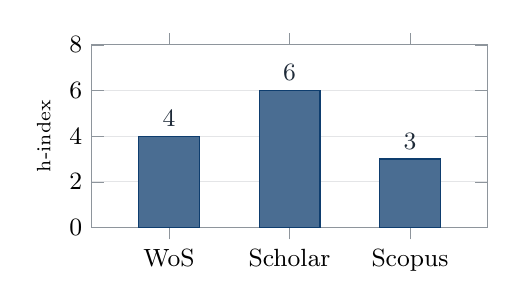
\begin{tikzpicture}
\begin{axis}[
    width=6.6cm, height=3.9cm,
    ybar, bar width=22pt,
    ymin=0, ymax=8, ytick={0,2,4,6,8},
    ylabel={\scriptsize h-index},
    symbolic x coords={WoS,Scholar,Scopus},
    xtick=data,
    nodes near coords, nodes near coords style={font=\small\bfseries,color=dark},
    tick label style={font=\small},
    axis line style={dark!50}, tick style={dark!50},
    enlarge x limits=0.32,
    ymajorgrids=true, grid style={dark!12},
]
\addplot+[fill=uaicblue!75,draw=uaicblue] coordinates {(WoS,4) (Scholar,6) (Scopus,3)};
\end{axis}
\end{tikzpicture}

\column{0.42\textwidth}
\begin{block}{\faAward\; Recunoaștere academică}
\footnotesize
\begin{itemize}\setlength\itemsep{0.4em}
  \item Membru în \textbf{comitete științifice internaționale}
  \item \textbf{10} din 18 articole ISI cu \textbf{factor de impact}
  \item Vizibilitate în WoS, Scopus, Google Scholar
\end{itemize}
\end{block}
\end{columns}
\end{frame}

% =====================================================
\section{Analiza SWOT a dezvoltării carierei academice}
% =====================================================

% ---- 3.0 SWOT overview ----
\begin{frame}{Analiza SWOT — privire de ansamblu}
\vspace{0.2em}
\centering
\begin{tikzpicture}[
  quad/.style={rectangle,rounded corners=10pt,minimum width=5.6cm,minimum height=2.7cm,
               inner sep=8pt,align=left,font=\footnotesize,line width=1pt,
               drop shadow={opacity=0.16,shadow xshift=1.2pt,shadow yshift=-1.2pt}},
  hd/.style={font=\small\bfseries}]
  % S
  \node[quad,draw=green,fill=green!8,text=dark] (S) at (-2.95,1.5)
    {\textcolor{green!65!black}{\faPlusCircle\; \textbf{Puncte forte}}\\[0.3em]
     Interdisciplinaritate $\cdot$ expertiză\\ aplicativă în volei de performanță\\ $\cdot$ activitate științifică solidă};
  % W
  \node[quad,draw=accent,fill=accent!8,text=dark] (W) at (2.95,1.5)
    {\textcolor{accent}{\faExclamationCircle\; \textbf{Puncte slabe}}\\[0.3em]
     Vizibilitate Q1/Q2 de crescut $\cdot$\\ optimizarea timpului $\cdot$ criterii\\ pentru conducere de doctorat};
  % O
  \node[quad,draw=uaicblue,fill=uaicblue!8,text=dark] (O) at (-2.95,-1.5)
    {\textcolor{uaicblue}{\faLightbulb\; \textbf{Oportunități}}\\[0.3em]
     Sănătate \& IA $\cdot$ finanțare\\ europeană $\cdot$ internaționalizare\\ $\cdot$ incluziune socială};
  % T
  \node[quad,draw=gold!85!black,fill=gold!12,text=dark] (T) at (2.95,-1.5)
    {\textcolor{gold!60!black}{\faBolt\; \textbf{Amenințări}}\\[0.3em]
     Competiție academică $\cdot$ declin\\ demografic $\cdot$ finanțare instabilă\\ $\cdot$ presiuni birocratice};
  % cruce centrală
  \draw[dark!25,line width=1pt] (0,2.95) -- (0,-2.95);
  \draw[dark!25,line width=1pt] (-5.9,0) -- (5.9,0);
  \node[circle,fill=white,draw=dark!30,line width=1pt,inner sep=2pt,font=\scriptsize\bfseries,text=dark] at (0,0){SWOT};
\end{tikzpicture}
\end{frame}

% ---- 3.1 Puncte forte ----
\begin{frame}{\faPlusCircle\; Puncte forte}
\vspace{0.4em}
\centering
\begin{tikzpicture}[card/.style={rectangle,rounded corners=10pt,minimum width=5.75cm,minimum height=1.7cm,
      inner sep=8pt,align=left,text width=5.25cm,font=\scriptsize,line width=0.9pt,
      drop shadow={opacity=0.15,shadow xshift=1pt,shadow yshift=-1pt}}]
  \node[card,draw=uaicblue,fill=uaicblue!8,text=dark] at (-3.1,1.95)
    {\textcolor{uaicblue}{\faProjectDiagram\; \textbf{Interdisciplinaritate}}\\[0.18em] Educație fizică $\cdot$ sport $\cdot$ sănătate $\cdot$ activitate adaptată $\cdot$ management};
  \node[card,draw=accent,fill=accent!8,text=dark] at (3.1,1.95)
    {\textcolor{accent}{\faVolleyballBall\; \textbf{Expertiză aplicativă}}\\[0.18em] Sport de performanță $\cdot$ volei de înalt nivel $\cdot$ transfer cercetare–practică};
  \node[card,draw=green,fill=green!8,text=dark] at (-3.1,0)
    {\textcolor{green!65!black}{\faChartLine\; \textbf{Activitate științifică}}\\[0.18em] 18 articole WoS (10 cu IF) $\cdot$ 25 BDI $\cdot$ conferințe și proiecte};
  \node[card,draw=teal,fill=teal!9,text=dark] at (3.1,0)
    {\textcolor{teal!72!black}{\faUniversity\; \textbf{Management universitar}}\\[0.18em] Director Extensia Chișinău $\cdot$ dezvoltare instituțională $\cdot$ evenimente};
  \node[card,draw=uaicsky,fill=uaicsky!10,text=dark] at (-3.1,-1.95)
    {\textcolor{uaicsky!85!black}{\faGlobeEurope\; \textbf{Internaționalizare}}\\[0.18em] 6 mobilități Erasmus+ $\cdot$ parteneriate academice $\cdot$ rețele internaționale};
  \node[card,draw=plum,fill=plum!9,text=dark] at (3.1,-1.95)
    {\textcolor{plum!80!black}{\faRocket\; \textbf{Dezvoltare viitoare}}\\[0.18em] Proiecte educaționale $\cdot$ cercetare $\cdot$ coordonare doctorală};
\end{tikzpicture}
\end{frame}

% ---- 3.2 Puncte slabe / consolidare ----
\begin{frame}{\faExclamationCircle\; Puncte slabe — direcții de consolidare}
\vspace{0.4em}
\centering
\begin{tikzpicture}[card/.style={rectangle,rounded corners=10pt,minimum width=5.75cm,minimum height=1.75cm,
      inner sep=8pt,align=left,text width=5.25cm,font=\scriptsize,line width=0.9pt,
      drop shadow={opacity=0.15,shadow xshift=1pt,shadow yshift=-1pt}}]
  \node[card,draw=accent,fill=accent!8,text=dark] at (-3.1,1.25)
    {\textcolor{accent}{\faChartBar\; \textbf{Vizibilitate internațională}}\\[0.18em] Publicații \textbf{Q1 și Q2} $\cdot$ articole \textbf{Open Access} $\cdot$ extinderea colaborărilor};
  \node[card,draw=gold!85!black,fill=gold!12,text=dark] at (3.1,1.25)
    {\textcolor{gold!60!black}{\faClock\; \textbf{Optimizarea timpului}}\\[0.18em] Echilibrarea activităților didactice, manageriale, administrative și de cercetare};
  \node[card,draw=teal,fill=teal!9,text=dark] at (-3.1,-0.7)
    {\textcolor{teal!72!black}{\faGlobe\; \textbf{Cercetare internațională}}\\[0.18em] Consorții europene $\cdot$ \textbf{Horizon Europe} \& Erasmus+ $\cdot$ infrastructură};
  \node[card,draw=uaicblue,fill=uaicblue!8,text=dark] at (3.1,-0.7)
    {\textcolor{uaicblue}{\faGraduationCap\; \textbf{Cariera academică}}\\[0.18em] Criterii \textbf{conducere de doctorat} $\cdot$ articol WoS Open Access};
  \node[rounded corners=8pt,fill=green!10,draw=green!50,line width=0.8pt,inner sep=8pt,
        font=\small,text=dark,text width=11.0cm,align=center] at (0,-2.55)
    {\textcolor{green!60!black}{\faRocket}\; \textit{Transformarea provocărilor actuale în \textbf{oportunități} de dezvoltare academică și instituțională.}};
\end{tikzpicture}
\end{frame}

% ---- 3.3 Oportunități ----
\begin{frame}{\faLightbulb\; Oportunități de dezvoltare}
\vspace{0.5em}
\centering
\begin{tikzpicture}[card/.style={rectangle,rounded corners=10pt,minimum width=5.7cm,minimum height=1.65cm,
      inner sep=8pt,align=left,text width=5.2cm,font=\footnotesize,line width=0.9pt,
      drop shadow={opacity=0.15,shadow xshift=1pt,shadow yshift=-1pt}}]
  \node[card,draw=green,fill=green!8,text=dark] (a) at (-3.1,1.95)
    {\textcolor{green!65!black}{\faHeartbeat\; \textbf{Sănătate și activitate fizică}}\\[0.15em] activitate fizică bazată pe dovezi $\cdot$ impact social};
  \node[card,draw=teal,fill=teal!9,text=dark] (b) at (3.1,1.95)
    {\textcolor{teal!72!black}{\faMicrochip\; \textbf{Digitalizare și IA}}\\[0.15em] monitorizarea performanței $\cdot$ intervenții personalizate};
  \node[card,draw=uaicblue,fill=uaicblue!8,text=dark] (c) at (-3.1,0)
    {\textcolor{uaicblue}{\faEuroSign\; \textbf{Finanțare europeană}}\\[0.15em] Horizon Europe $\cdot$ Erasmus+ $\cdot$ cercetare și inovare};
  \node[card,draw=uaicsky,fill=uaicsky!10,text=dark] (d) at (3.1,0)
    {\textcolor{uaicsky!85!black}{\faGlobeEurope\; \textbf{Internaționalizare}}\\[0.15em] dublă diplomă $\cdot$ cooperare R. Moldova \& Ucraina};
  \node[card,draw=plum,fill=plum!9,text=dark,minimum width=11.6cm,text width=11.0cm,align=center] (e) at (0,-1.95)
    {\textcolor{plum!80!black}{\faWheelchair\; \textbf{Incluziune și activitate fizică adaptată}} $\;\cdot\;$ sport și incluziune socială $\cdot$ cercetare cu impact comunitar};
\end{tikzpicture}
\end{frame}

% ---- 3.4 Amenințări ----
\begin{frame}{\faBolt\; Amenințări și provocări}
\vspace{0.5em}
\begin{columns}[T,onlytextwidth]
\column{0.5\textwidth}
\footnotesize
\begin{itemize}\setlength\itemsep{0.7em}
  \item \textcolor{gold!60!black}{\faTrophy}\; \textbf{Competiția academică internațională}\\ \sub{standarde de performanță în creștere, competiție pentru granturi}
  \item \textcolor{gold!60!black}{\faUsers}\; \textbf{Evoluții demografice}\\ \sub{scăderea populației școlare și universitare}
  \item \textcolor{gold!60!black}{\faCoins}\; \textbf{Finanțarea cercetării}\\ \sub{instabilitatea mecanismelor de finanțare}
\end{itemize}
\column{0.5\textwidth}
\footnotesize
\begin{itemize}\setlength\itemsep{0.7em}
  \item \textcolor{gold!60!black}{\faLaptopCode}\; \textbf{Transformări tehnologice accelerate}\\ \sub{actualizarea continuă a competențelor}
  \item \textcolor{gold!60!black}{\faFileSignature}\; \textbf{Presiuni administrative și birocratice}\\ \sub{mai puțin timp pentru cercetare strategică}
\end{itemize}
\vspace{0.4em}
\begin{alertblock}{\faBullseye\; Răspuns strategic}
\footnotesize Adaptabilitate $\cdot$ internaționalizare $\cdot$ inovare $\cdot$ dezvoltare continuă.
\end{alertblock}
\end{columns}
\end{frame}

% =====================================================
\section{Direcții strategice de dezvoltare viitoare}
% =====================================================

% ---- 4.1 Obiectiv + direcții de cercetare ----
\begin{frame}{Obiectiv strategic și direcții de cercetare}
\vspace{0.2em}
\begin{block}{\faBullseye\; Obiectiv strategic}
\footnotesize Integrare activă în \textbf{Școala Doctorală} $\cdot$ contribuție la dezvoltarea cercetării și a mediului academic $\cdot$ creșterea vizibilității naționale și internaționale
\end{block}
\vspace{0.2em}
\centering
\begin{tikzpicture}[dir/.style={rectangle,rounded corners=8pt,minimum width=3.55cm,minimum height=1.35cm,
      inner sep=5pt,align=center,font=\scriptsize,line width=0.8pt,
      drop shadow={opacity=0.14,shadow xshift=1pt,shadow yshift=-1pt}}]
  \node[dir,draw=green,fill=green!8,text=dark] at (-4,0.85){\textcolor{green!65!black}{\faHeartbeat}\\ \textbf{Activitate fizică}\\ \textbf{și sănătate}};
  \node[dir,draw=plum,fill=plum!9,text=dark] at (0,0.85){\textcolor{plum!80!black}{\faWheelchair}\\ \textbf{Activitate adaptată}\\ \textbf{și incluziune}};
  \node[dir,draw=accent,fill=accent!8,text=dark] at (4,0.85){\textcolor{accent}{\faVolleyballBall}\\ \textbf{Performanță și}\\ \textbf{optimizarea antren.}};
  \node[dir,draw=teal,fill=teal!9,text=dark] at (-4,-0.85){\textcolor{teal!72!black}{\faMicrochip}\\ \textbf{IA și tehnologii}\\ \textbf{digitale în sport}};
  \node[dir,draw=uaicblue,fill=uaicblue!8,text=dark] at (0,-0.85){\textcolor{uaicblue}{\faChartLine}\\ \textbf{Monitorizarea}\\ \textbf{performanței motrice}};
  \node[dir,draw=gold!85!black,fill=gold!12,text=dark] at (4,-0.85){\textcolor{gold!60!black}{\faBookOpen}\\ \textbf{Programe educ.}\\ \textbf{bazate pe dovezi}};
\end{tikzpicture}
\end{frame}

% ---- 4.2 Internaționalizare + Chișinău ----
\begin{frame}{Internaționalizare și dezvoltare instituțională}
\vspace{0.4em}
\begin{columns}[T,onlytextwidth]
\column{0.5\textwidth}
\begin{block}{\faGlobeEurope\; Internaționalizare}
\footnotesize
\begin{itemize}\setlength\itemsep{0.45em}
  \item Parteneriate academice internaționale
  \item Proiecte europene și consorții de cercetare
  \item Mobilități și colaborări interdisciplinare
\end{itemize}
\end{block}
\column{0.5\textwidth}
\begin{exampleblock}{\faMapMarker\; Extensia UAIC Chișinău \;\faFlag}
\footnotesize
\begin{itemize}\setlength\itemsep{0.45em}
  \item Cooperare academică transfrontalieră
  \item Dezvoltarea programelor educaționale
  \item Extinderea colaborărilor științifice
\end{itemize}
\end{exampleblock}
\end{columns}
\vspace{0.5em}
\begin{center}

\begin{tikzpicture}\node[rounded corners=9pt,fill=uaicblue!8,draw=uaicblue!45,line width=0.9pt,inner sep=9pt,
  text=dark,font=\small,text width=11.0cm,align=center]{%
  \faHandshake\; \textit{Cooperare cu universități din \textbf{Republica Moldova} și \textbf{Ucraina} — pol regional de excelență.}};\end{tikzpicture}
\end{center}
\end{frame}

% ---- 4.3 Viziune ----
\begin{frame}{Viziune}
\vspace{0.6em}
\centering
\begin{tikzpicture}[every node/.style={align=center}]
  \foreach \i/\ic/\lab/\col in {0/\faFlask/{Cercetare}/uaicblue,1/\faGraduationCap/{Educație}/green,
       2/\faUniversity/{Management}/accent,3/\faGlobeEurope/{Cooperare intl.}/teal}{
    \node[circle,fill=\col!12,draw=\col,line width=1.1pt,minimum size=1.9cm,
          drop shadow={opacity=0.18,shadow xshift=1.2pt,shadow yshift=-1.2pt}] (c\i) at (\i*3.2,0)
      {\begin{tabular}{c}{\large\textcolor{\col}{\ic}}\\[0.15em]\footnotesize\textbf{\textcolor{\col!75!black}{\lab}}\end{tabular}};
  }
  \foreach \i in {0,1,2}{\draw[-{Stealth[length=3mm]},dark!35,line width=1.1pt] (c\i.east) -- (c\the\numexpr\i+1\relax.west);}
\end{tikzpicture}

\vspace{1.1em}

\begin{tikzpicture}
\node[rounded corners=10pt,fill=accent!10,draw=accent!50,line width=1pt,inner sep=11pt,
      text=dark,font=\normalsize,text width=11.5cm,align=center]{%
  \faRocket\; Contribuții la promovarea \textbf{performanței sportive}, a \textbf{sănătății} și a \textbf{incluziunii sociale}, prin cercetare, educație și cooperare internațională.};
\end{tikzpicture}
\end{frame}

% =====================================================
%  SLIDE FINAL
% =====================================================
{
\setbeamertemplate{footline}{}
\begin{frame}[plain]

\begin{tikzpicture}[overlay,remember picture]
  \fill[uaicblue] (current page.north west) rectangle (current page.south east);
  \begin{scope}[shift={([xshift=-1.6cm,yshift=-1.6cm]current page.north east)}]
    \foreach \r in {0.6,1.2,...,3.8} \draw[white,opacity=0.09,line width=1.2pt] (0,0) circle (\r);
    \fill[white,opacity=0.18] (0,0) circle (0.42);
  \end{scope}
  \begin{scope}[shift={([xshift=1.9cm,yshift=1.7cm]current page.south west)}]
    \foreach \r in {0.4,0.9,...,3.0} \draw[white,opacity=0.09,line width=1.2pt] (0,0) circle (\r);
  \end{scope}
  \node[text=white,opacity=0.12,font=\fontsize{40}{40}\selectfont] at ([xshift=-2.6cm,yshift=2.1cm]current page.south east){\faVolleyballBall};
  \node[text=white,opacity=0.10,font=\fontsize{30}{30}\selectfont] at ([xshift=-4.4cm,yshift=2.6cm]current page.south east){\faHeartbeat};

  \node[text=white,font=\fontsize{52}{52}\selectfont\bfseries,anchor=center]
    at ([yshift=0.85cm]current page.center) {Vă mulțumesc!};
  \draw[accent,line width=3pt,line cap=round]
    ([yshift=-0.6cm,xshift=-1.7cm]current page.center) -- ([yshift=-0.6cm,xshift=1.7cm]current page.center);
  \node[text=white!88,font=\Large\itshape,anchor=center] at ([yshift=-1.3cm]current page.center) {Întrebări și discuții};

  \node[text=white!80,font=\small,anchor=center,align=center] at ([yshift=-2.6cm]current page.center)
    {\faUserGraduate\; Lect. Univ. Dr. Puni Alexandru-Rareș \;\;$\cdot$\;\; \faUniversity\; UAIC Iași — Facultatea de Educație Fizică și Sport};
\end{tikzpicture}
\end{frame}
}

\end{document}
